\documentclass[11pt,a4paper]{article}

% ---------------- PACKAGES ----------------
\usepackage[utf8]{inputenc}
\usepackage[T1]{fontenc}
\usepackage[english]{babel}
\usepackage{amsmath, amssymb}
\usepackage{siunitx}
\usepackage{geometry}
\usepackage{multicol}
\usepackage{tcolorbox}
\usepackage{tikz}
\usepackage{xcolor}
\usepackage{fancyhdr}

\geometry{margin=2cm}
\pagestyle{fancy}
\fancyhf{}
\lhead{\textbf{Power and Energy}}
\rhead{\thepage}

% ---------------- COLORS ----------------
\definecolor{energyblue}{RGB}{30,80,160}
\definecolor{powerred}{RGB}{180,50,50}
\definecolor{warningred}{RGB}{200,30,30}
\definecolor{graybg}{RGB}{245,245,245}

% ---------------- TCOLORBOX ----------------
\tcbset{
  sharp corners,
  colback=white,
  colframe=black!60,
  boxrule=0.8pt,
  left=6pt, right=6pt, top=4pt, bottom=4pt
}

\newcommand{\theorybox}[2]{
\begin{tcolorbox}[title=\textbf{#1}]
#2
\end{tcolorbox}
}

% ---------------- EXERCISE GRIDS ----------------
\newcommand{\fullgrid}{
\vfill
\begin{center}

\begin{tikzpicture}[scale=0.9]
\draw[step=0.5cm,gray!30,very thin] (0,0) grid (18,22);
\end{tikzpicture}
\end{center}
\vfill
}

\newcommand{\threequartergrid}{
\vfill
\begin{center}

\begin{tikzpicture}[scale=0.9]
\draw[step=0.5cm,gray!30,very thin] (0,0) grid (18,18);
\end{tikzpicture}
\end{center}
\vfill
}

\begin{document}

% =================================================
% TITLE PAGE
% =================================================


\section*{Pumped storage and energy economics}

This exercise studies the simplified operation of the pumped-storage
hydroelectric system between the Hongrin reservoir and Lake Léman.

\begin{figure}
    \centering
    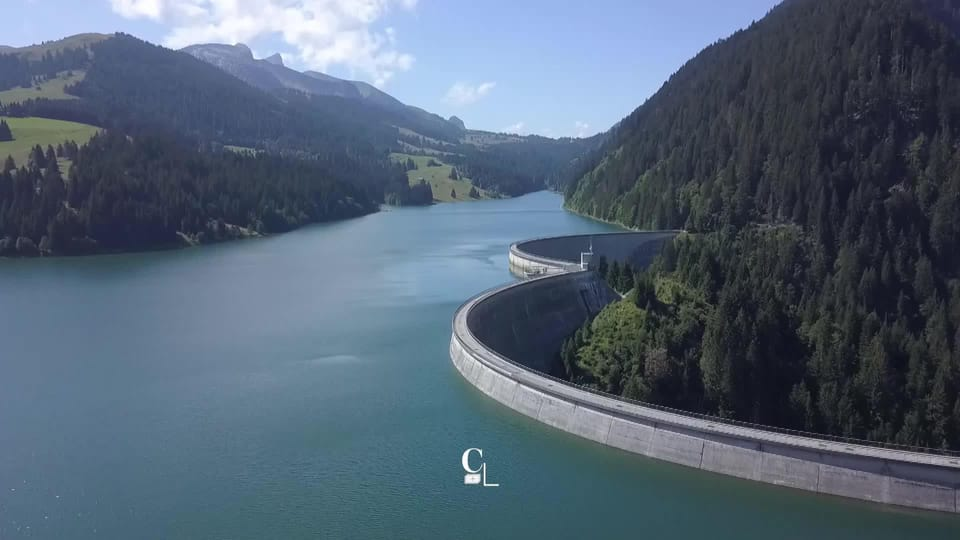
\includegraphics[width=0.75\linewidth]{barage.jpeg}
    \caption{Le Barrage de l'Hongrin, source : RTS}
\end{figure}

The system works as follows:

\begin{itemize}
\item At night, electricity is cheap and pumps are used to raise water
from Lake Léman to the Hongrin reservoir.
\item During the day, the stored water flows downhill through turbines
to generate electricity when electricity prices are higher.
\end{itemize}

This allows energy to be \textbf{stored and resold later}.

Electricity price:
\begin{itemize}
\item Night (00h00 -- 07h00): $15\,\si{ct/kWh}$
\item Day (07h00 -- 24h00): $35\,\si{ct/kWh}$
\end{itemize}

System characteristics:

\begin{itemize}
\item Surface of the Hongrin lake: $1.6\,\si{km^2}$
\item Average depth of the lake: $30\,\si{m}$
\item Height difference with Lake Léman: $900\,\si{m}$

\item Maximum turbine power: $500\,\si{MW}$
\item Maximum pump power: $400\,\si{MW}$

\item Turbine + generator efficiency: $90\%$
\item Pump efficiency: $80\%$

\item Annual water inflow to the reservoir:
$150\,\text{million } \si{m^3 / year}$

\item Average household consumption:
$4500\,\si{kWh/year}$

\item Electric car consumption:
$150\,\si{Wh/km}$
\end{itemize}

All calculations must be done in \textbf{SI units}.

\newpage
% -------------------------------------------------
\subsection*{Part A - Volume of the reservoir}

We start by estimating the volume of water stored in the lake.

\begin{itemize}

\item Convert the surface area of the lake from $\si{km^2}$ to $\si{m^2}$.

\item Identify the average depth of the lake.

\item Compute the total volume of water stored in the reservoir.

\item Express the result in $\si{m^3}$.

\end{itemize}

\threequartergrid

% -------------------------------------------------
\newpage
\subsection*{Part B - Potential energy stored in the lake}

The water in the reservoir is located about $900\,\si{m}$ above Lake Léman.

This means the water contains gravitational potential energy.

\begin{itemize}

\item Determine the total mass of water contained in the reservoir
(using the density of water).

\item Identify the height difference between the two lakes.

\item Compute the total gravitational energy stored in the reservoir.

\item Express the result in joules.

\item Convert this energy into $\si{kWh}$.

\end{itemize}

\threequartergrid

% -------------------------------------------------
\newpage
\subsection*{Part C - Maximum electrical power generation}

When the water flows downhill, turbines generate electricity.

\begin{itemize}

\item Identify the maximum mechanical power available from the turbine.

\item Take the turbine and generator efficiency into account.

\item Compute the maximum electrical power delivered to the grid.

\item Express the result in $\si{MW}$.

\end{itemize}

\threequartergrid

% -------------------------------------------------
\newpage
\subsection*{Part D - Daily energy production}

Assume the turbines operate at maximum power during the day.

\begin{itemize}

\item Determine the duration of the daytime electricity market.

\item Compute the maximum electrical energy that can be produced
during one day.

\item Express the result in $\si{kWh}$.

\end{itemize}

\threequartergrid

% -------------------------------------------------
\newpage
\subsection*{Part E - Pumping energy during the night}

At night, electricity is used to pump water back to the reservoir.

\begin{itemize}

\item Determine the duration of the night period.

\item Identify the maximum electrical power of the pumps.

\item Compute the electrical energy used by the pumps each night.

\item Take the pump efficiency into account and determine the
gravitational energy actually stored in the water.

\end{itemize}

\threequartergrid

% -------------------------------------------------
\newpage
\subsection*{Part F - Daily economic profit}

The goal of pumped storage is to buy electricity when it is cheap
and sell it when it is expensive.

\begin{itemize}

\item Compute the cost of the electricity used for pumping during the night.

\item Compute the value of the electricity sold during the day.

\item Take the efficiencies into account.

\item Compute the net profit for one full daily cycle.

\item Express the result in Swiss francs per day.

\end{itemize}

\threequartergrid

% -------------------------------------------------
\newpage
\subsection*{Part G - How many homes can be powered?}

We now estimate how many households can be supplied.

\begin{itemize}

\item Use the annual water inflow of the reservoir.

\item Compute the total gravitational energy available each year.

\item Take turbine efficiency into account to determine the electrical
energy produced.

\item Convert the result into $\si{kWh/year}$.

\item Compare this value with the annual electricity consumption
of one household.

\item Determine how many households could be supplied.

\end{itemize}

\threequartergrid

% -------------------------------------------------
\newpage
\subsection*{Part H - Energy equivalent in electric cars}

Finally, we compare this energy with electric mobility.

\begin{itemize}

\item Use the total electrical energy stored in the lake.

\item Convert the energy into watt-hours.

\item Use the average consumption of an electric car.

\item Compute the total distance that could be driven using
this stored energy.

\item Express the result in kilometers.

\end{itemize}

\threequartergrid

\end{document}

